%- [X] mDL [AFONSO]
%   - [X] Funcionalidades (API)
%       - [X] __init__(self, data=None)
%       - [X] load(self)
%       - [X] save(self)
%       - [X] set_permissions(self, allow)
%       - [X] add_permissions(self, allow)
%       - [?] get_data(self, data_group_tags)
%       - [X] get_signature(self)
%       - [X] get_digests(self, data_groups)
%       - [X] get_available_data_groups(self)
%       - [X] get_data_hex(self, data_group_tags)
%   - [X] Exemplo de utilização

A aplicação mDL tem como objetivo incorporar todos os componentes anteriormente descritos, de forma a fornecer as funcionalidades que permitem animar a interação com o mDL\@.

\subsubsection{Funcionalidades (API)}

Primeiramente, é necessário inicializar o mDL (\texttt{\_\_init\_\_}). Para tal, à semelhança de outras classes da ferramenta, é possível passar um JSON com os dados, ou simplesmente deixar que o mDL carregue os dados que guardou na última utilização (\texttt{load}). Esta última opção é apenas possível se já tiver sido usada a função \texttt{save}, que persiste os dados (codificados em ASN1) do mDL em ficheiros. Na prática, tanto o \texttt{load} como o \texttt{save} realizam as suas operações delegando a tarefa a cada um dos grupos de dados.

\begin{Verbatim}[frame=single, framerule=0.5mm]
def load(self):
    self.dg1 = dg1.DG1('./data_groups/asn1_hex_data/dg1.txt')
    self.dg6 = dg6.DG6('./data_groups/asn1_hex_data/dg6.txt')
    (...)
\end{Verbatim}

\begin{Verbatim}[frame=single, framerule=0.5mm]
def save(self):
    self.dg1.save('./data_groups/asn1_hex_data/dg1.txt') 
    self.dg6.save('./data_groups/asn1_hex_data/dg6.txt') 
    (...)
\end{Verbatim}

Mais ainda, uma parte fundamental do mDL é a possibilidade de definir quais os grupos de dados aos quais se tem acesso. Para tal, são utilizadas as funcionalidades de \texttt{set\_permissions} e \texttt{add\_permissions}, oferecidas pela classe \texttt{ef\_groupAccess}, para definir permissões ou permitir novos grupos de dados, respetivamente. Importa salientar que o documento ISO que serviu de referência para a realização deste projeto, não afirma de forma clara, a que é que se deve aplicar as permissões mencionadas anteriormente. No entanto, é referido no ISO que os valores de hash, utilizados na autenticação passiva, são sobre o DG completo (Pág. 20 da parte 3). Desta forma, a validação efetuada pelo verificador implica que este tenha acesso a todos os elementos do DG, de forma a reconstruir o \textit{digest}, mesmo que só tenha permissão para alguns. Tendo em conta este caso, considerou-se que as permissões são estabelecidas por DG e não para os campos de cada DG individualmente.

\begin{Verbatim}[frame=single, framerule=0.5mm]
def set_permissions(self, allow):
	self.ef_groupAccess.set_permissions(allow)
\end{Verbatim}

\begin{Verbatim}[frame=single, framerule=0.5mm]
def add_permissions(self, allow):
	self.ef_groupAccess.add_permissions(allow)
\end{Verbatim}

Outra funcionalidade disponibilizada está relacionada com a necessidade de autenticar a origem da informação da mDL\@. Para tal, o processo de autenticação passiva incorpora um mecanismo de validação da assinatura dos dados do mDL\@. De forma a disponibilizar esta funcionalidade tem-se a função \texttt{get\_signature} que devolve as informações necessárias para que o leitor mDL possa realizar a validação. Adicionalmente, o processo de autenticação passiva envolve a validação dos valores de hash dos dados de cada DG\@. Esses mesmo valores também são incorporados na resposta devolvida pela função \texttt{get\_sod\_data\_hex}.

\begin{Verbatim}[frame=single, framerule=0.5mm]
def get_sod_data_hex(self):
    return self.ef_sod.encode()
\end{Verbatim}

A função \texttt{get\_available\_data\_groups} surge como uma necessidade na implementação do processo de transação existente entre um dispositivo mDL e um leitor mDL\@. Efetivamente, o primeiro passo do mDL envolve a pré-seleção dos dados que podem ser partilhados. Desta forma, a função anterior é necessária para se averiguar quais os DG's que se encontram no mDL, para que, posteriormente, se possa definir as respetivas permissões.

\begin{Verbatim}[frame=single, framerule=0.5mm]
def get_available_data_groups(self):
	return self.ef_com.get_data()['tag_list']
\end{Verbatim}

Por fim, tem-se a função \texttt{get\_data\_hex} que permite que os dados do mDL, codificados ASN1, sejam acedidos. Na prática a função percorre as tags dos grupos de dados recebidas como argumento e verifica, consultando o EF.GroupAccess se o DG pode ser acedido. Se tal for verdade, então o conteúdo do DG, codificado em ASN1, é concatenado com o restante \textit{output} e é retornado.

\begin{Verbatim}[frame=single, framerule=0.5mm]
def get_data_hex(self, data_group_tags):
	hex_data = ''
	for tag in data_group_tags:
		num_dg = self.TAGS[tag]
		if self.ef_groupAccess.is_allowed(num_dg):
			hex_data += self.get_dg(num_dg).encode()
	return hex_data
\end{Verbatim}

Adicionalmente, também é possível aceder aos dados de forma estruturada (sem ser codificados em hexadecimal), através da função \texttt{get\_data}.


\subsubsection{Exemplo de utilização}

Um possível exemplo de utilização envolve a execução de uma transação entre um dispositivo mDL e um leitor mDL\@. Para tal, foram criadas duas classes: \texttt{mDL\_transaction} e \texttt{mDL\_simulator}. Por um lado, a primeira tem como objetivo utilizar a classe \texttt{mDL} e implementar os passos que possam existir numa dada transação. Por outro lado, a segunda tem como objetivo animar a transação entre os dois intervenientes.

A classe \texttt{mDL\_transaction} possui a seguinte API:

\begin{itemize}
	\item \texttt{\_\_init\_\_}: inicializa o mDL.
	\item \texttt{open}: anima o processo de abertura do mDL
	\item \texttt{preselect}: permite que o utilizador defina as permissões para os DG's existentes.
	\item \texttt{request\_additional\_data}: permite que seja requerido acesso a determinados DG's.
	\item \texttt{transfer\_data}: devolve os dados do mDL requeridos.
\end{itemize}

A título exemplificativo, o \texttt{mDL\_simulator} assume a seguinte transação:

\begin{Verbatim}[frame=single, framerule=0.5mm]
(...) # Carregamos do ficheiro JSON com os dados
MDLT = mDL_transaction(DATA)
MDLT.open()
MDLT.request_additional_data(['61', '62'])
transfer_data = MDLT.transfer_data(['61', '62'])
transfer_sod_data = MDLT.transfer_sod()

dg1 = dg1.DG1(transfer_data[1])
dg10 = dg10.DG10(transfer_data[10])
dgs = {1: dg1, 10: dg10}
transfer_digests = calculate_digests(dgs, transfer_sod_data['digestAlgorithm'])

(...) # Cálculo do valor dos digests dos DG's que se pretende aceder

digest1 = transfer_sod_data['dataGroupHash'][0]['dataGroupHashValue']
digest10 = transfer_sod_data['dataGroupHash'][2]['dataGroupHashValue']

(...) # Concatenação dos valores dos digests recebidos do mDL

print('DIGESTS VALIDATION:',
        transfer_digests[1] == digest1 and\
        transfer_digests[10] == digest10)
print('SIGNATURE VALIDATION:',
    verify_signature(
        sod_digests,
        bytes(transfer_sod_data['certificate']),
        bytes(transfer_sod_data['signature']),
        transfer_sod_data['signatureAlgorithm']
    ))
\end{Verbatim}

De forma, a popular o mDL é usado o seguinte ficheiro JSON:

\begin{lstlisting}[language=json]
{
    "dg1": {
        "family_name": "Smithe Williams",
        "name": "Alexander George Thomas",
        "date_of_birth": "19700301",
        "date_of_issue": "20020915",
        "date_of_expiry": "20070930",
        "issuing_country": "JPN",
        "issuing_authority": "HOKKAIDO PREFECTURAL POLICE ASAHIKAWA AREA SAFETY PUBLIC",
        "license_number": "A290654395164273X",
        "number_of_entries": 2,
        "categories_of_vehicles": [
            "C1;20000315;20100314;S01;<=;38303030",
            "C1;20000315;20100314;S01;<=;38303030"
        ]
    },
    "dg6": {
        "biometric_templates": [
            {
                "version": 257,
                "bdb_owner": 257,
                "bdb_type": 8,
                "bdb": "picture.jpg"
            },
            {
                "version": 257,
                "bdb_owner": 257,
                "bdb_type": 8,
                "bdb": "picture.jpg"
            }
        ],
        "number_of_entries": 2
    },
    "dg10": {
        "version": "1",
        "last_update": "20130115000000",
        "expiration_date": "20130314235959",
        "next_update": "20130122000000",
        "management_info": "info"
    },
    "ef_groupAccess": {
        "6": "75"
    },
    "ef_com": {
        "version": "0100",
        "tag_list": ["61", "75", "62"]
    },
    "ef_sod": {
        "digestAlgorithm": "id-sha256",
        "signatureAlgorithm": "id-pk-RSA-PSS-SHA256",
        "certificate": "certificates/certificate.der",
        "signature": "certificates/key.der"
    }
}
\end{lstlisting}

Além de popular os diferentes constituintes do mDL, o JSON apenas permite o acesso ao DG6 através do campo \texttt{ef\_groupAccess}.

De seguida, encontra-se um exemplo de simulação, onde é feito uma correlação entre a interação e o processo de transação descrito no ISO.

\begin{figure}[H]
    \centering
    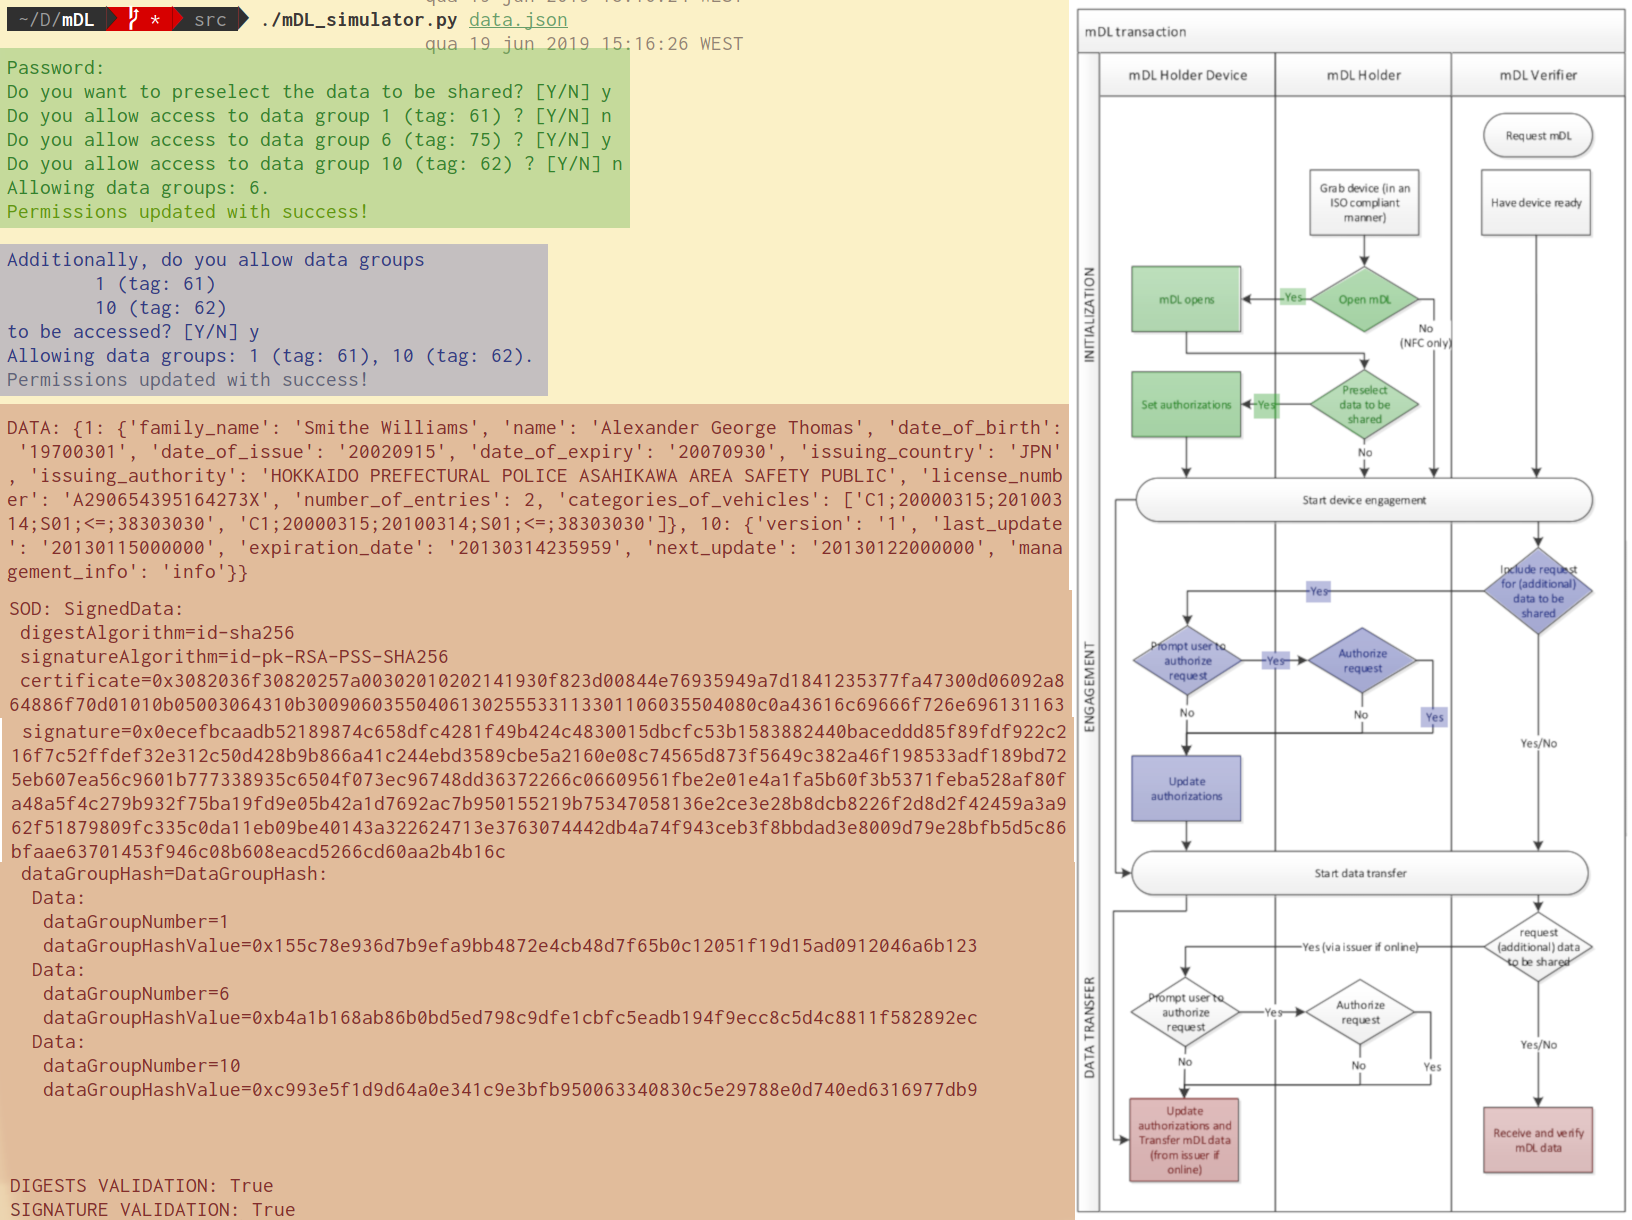
\includegraphics[width=0.95\textwidth]{working_example2.png}
    \caption{Exemplo de utilização do mDL.}
	\label{fig:working_example2}
\end{figure}

Neste exemplo o utilizador aceita pre-selecionar os DG's que pretende permitir o acesso, sendo que apenas dá permissão ao DG6. De seguida, é requirido que seja dada permissão de acesso ao DG1 e DG10. O utilizador aceita e os dados são transferidos para o leitor do mDL, para que este possa prosseguir com a operação.

Importa realçar que o processo aqui descrito, que corresponde ao objectivo deste projeto, não envolve a componente de validação descrita no ISO do mDL\@. No entanto, esta foi adicionada de forma redimentar de forma a demonstrar o raciocínio necessário no momento de validção. Nesta pequena demonstração foram usados métodos e classes utilizados pelo mDL e, desta forma, teriam que ser reescritos pela entidade verificadora de forma a realizar a verificação de forma totalmente independente do mDL.
